% Shielding, chased to Maxwell: the full tower.
% Maxwell's two source equations -> shared 1/rho Green's function -> D_ab (waist) ->
% fork into magnetic/electrical doorways -> funnel into shielding.
% Compile: pdflatex -interaction=nonstopmode
\documentclass[border=16pt]{standalone}
\usepackage{amsmath}
\usepackage{tikz}
\usetikzlibrary{positioning,arrows.meta,calc,backgrounds}

\definecolor{ink}{RGB}{45,55,70}
\definecolor{cLaw}{RGB}{238,240,244}
\definecolor{tMag}{RGB}{42,84,140}
\definecolor{tElec}{RGB}{172,96,34}
\definecolor{tObs}{RGB}{40,110,55}
\definecolor{note}{RGB}{105,105,115}

\begin{document}
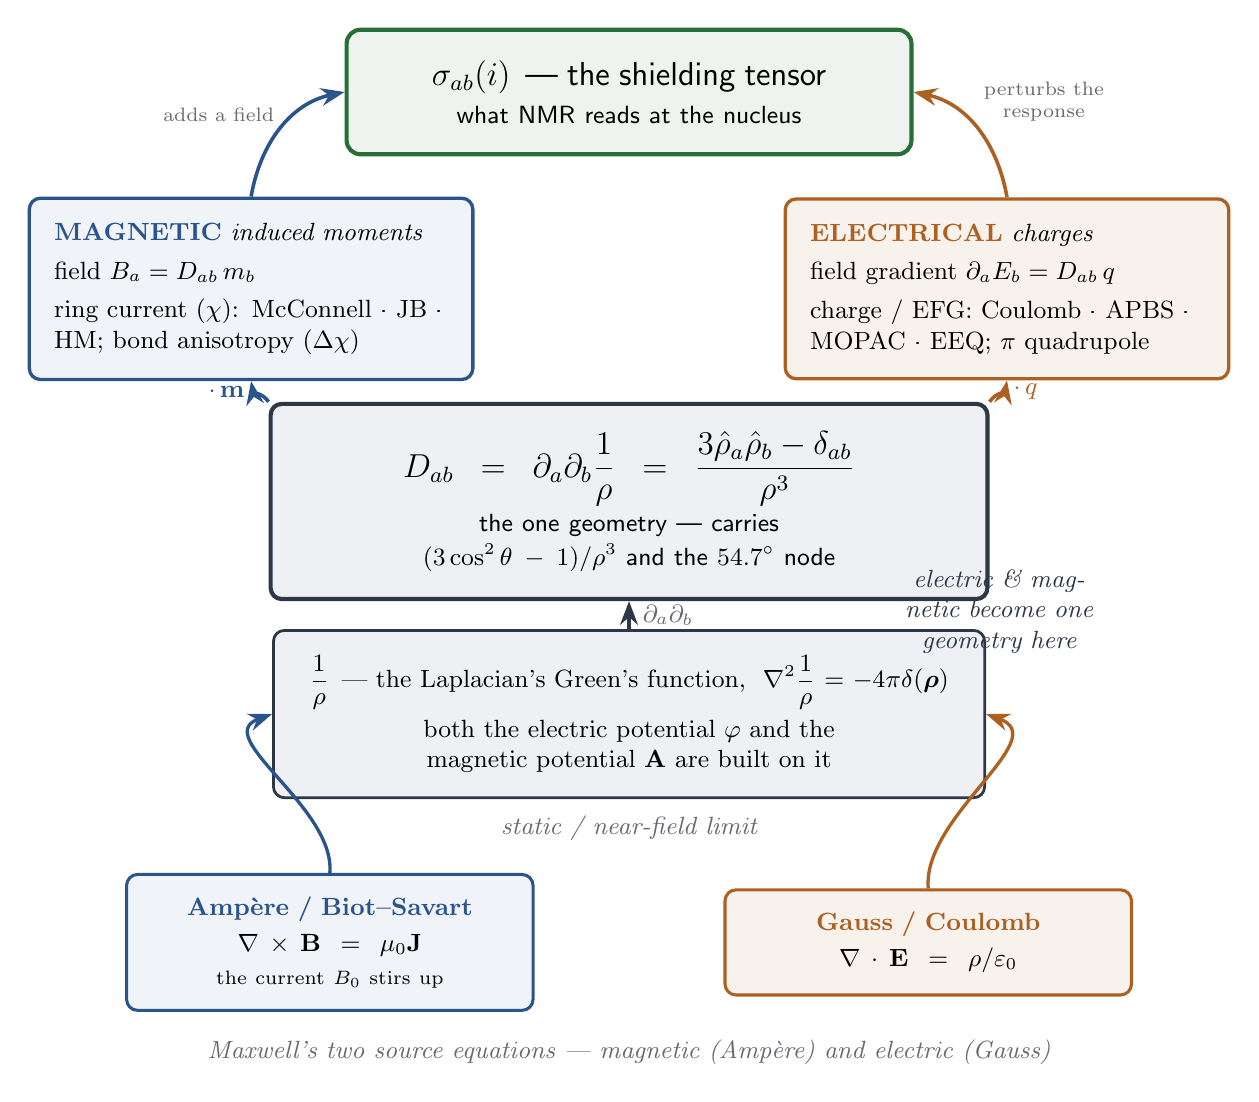
\begin{tikzpicture}[
  font=\sffamily,
  >={Stealth[length=3mm]},
  obs/.style={rounded corners=5pt, draw=tObs, line width=1.5pt, fill=tObs!8, align=center, inner sep=11pt, text width=6.4cm},
  mag/.style={rounded corners=4pt, draw=tMag, line width=1.2pt, fill=tMag!7, align=left, inner sep=9pt, text width=5.0cm, font=\small},
  elec/.style={rounded corners=4pt, draw=tElec, line width=1.2pt, fill=tElec!8, align=left, inner sep=9pt, text width=5.0cm, font=\small},
  ker/.style={rounded corners=4pt, draw=ink, line width=1.5pt, fill=cLaw, align=center, inner sep=10pt, text width=8.4cm},
  grn/.style={rounded corners=4pt, draw=ink, line width=1pt, fill=cLaw, align=center, inner sep=9pt, text width=8.4cm, font=\small},
  leg/.style={rounded corners=4pt, line width=1.1pt, align=center, inner sep=8pt, text width=4.6cm, font=\small},
]

% ---- the observable (apex) ----
\node[obs] (OBS) at (0,6.2) {%
  {\large $\sigma_{ab}(i)$\, --- the shielding tensor}\\[2pt]
  {\small what NMR reads at the nucleus}};

% ---- the two doorways ----
\node[mag] (MAG) at (-4.8,3.7) {%
  {\bfseries\textcolor{tMag}{MAGNETIC}}\ {\small\itshape induced moments}\\[3pt]
  field\ $B_a=D_{ab}\,m_b$\\[3pt]
  {\small ring current ($\chi$): McConnell \textperiodcentered\ JB \textperiodcentered\ HM; bond anisotropy ($\Delta\chi$)}};

\node[elec] (ELEC) at (4.8,3.7) {%
  {\bfseries\textcolor{tElec}{ELECTRICAL}}\ {\small\itshape charges}\\[3pt]
  field gradient\ $\partial_a E_b=D_{ab}\,q$\\[3pt]
  {\small charge / EFG: Coulomb \textperiodcentered\ APBS \textperiodcentered\ MOPAC \textperiodcentered\ EEQ; $\pi$ quadrupole}};

% ---- the waist: the one kernel ----
\node[ker] (DAB) at (0,1.0) {%
  {\large $\displaystyle D_{ab}=\partial_a\partial_b\frac{1}{\rho}=\frac{3\hat\rho_a\hat\rho_b-\delta_{ab}}{\rho^{3}}$}\\[2pt]
  {\small the one geometry --- carries $(3\cos^2\theta-1)/\rho^3$ and the $54.7^\circ$ node}};

% ---- the shared Green's function ----
\node[grn] (GRN) at (0,-1.7) {%
  $\dfrac{1}{\rho}$\, --- the Laplacian's Green's function,\ \ $\nabla^2\dfrac{1}{\rho}=-4\pi\delta(\boldsymbol\rho)$\\[3pt]
  {\small both the electric potential $\varphi$ and the magnetic potential $\mathbf A$ are built on it}};

% ---- Maxwell's two source equations (root) ----
\node[leg, draw=tMag, fill=tMag!7] (AMP) at (-3.8,-4.6) {%
  {\bfseries\textcolor{tMag}{Amp\`ere / Biot--Savart}}\\[2pt]
  $\nabla\times\mathbf B=\mu_0\mathbf J$\\[1pt]
  {\scriptsize the current $B_0$ stirs up}};

\node[leg, draw=tElec, fill=tElec!8] (GAU) at (3.8,-4.6) {%
  {\bfseries\textcolor{tElec}{Gauss / Coulomb}}\\[2pt]
  $\nabla\cdot\mathbf E=\rho/\varepsilon_0$};

\node[font=\small\itshape, text=note] (MX) at (0,-6.0) {Maxwell's two source equations --- magnetic (Amp\`ere) and electric (Gauss)};

% ============ arrows ============
% Maxwell -> Green's function (converge)
\draw[->, line width=1.2pt, tMag] (AMP.north) to[out=85,in=200] (GRN.west);
\draw[->, line width=1.2pt, tElec] (GAU.north) to[out=95,in=-20] (GRN.east);
\node[font=\small\itshape, text=note] at (0,-3.15) {static / near-field limit};

% Green's function -> kernel
\draw[->, line width=1.3pt, ink] (GRN.north) -- node[right=1pt, font=\small, text=note]{$\partial_a\partial_b$} (DAB.south);

% kernel forks
\draw[->, line width=1.3pt, tMag] (DAB.north west) to[out=125,in=-80]
   node[midway, left=1pt, font=\small, text=tMag]{$\cdot\,\mathbf m$} (MAG.south);
\draw[->, line width=1.3pt, tElec] (DAB.north east) to[out=55,in=-100]
   node[midway, right=1pt, font=\small, text=tElec]{$\cdot\,q$} (ELEC.south);

% doorways funnel into shielding
\draw[->, line width=1.3pt, tMag] (MAG.north) to[out=80,in=192]
   node[midway, above left=-2pt, font=\scriptsize, text=note, align=center]{adds a field} (OBS.west);
\draw[->, line width=1.3pt, tElec] (ELEC.north) to[out=100,in=-12]
   node[midway, above right=-2pt, font=\scriptsize, text=note, align=center]{perturbs the\\ response} (OBS.east);

% waist annotation
\node[font=\small\itshape, text=ink, align=center, text width=3.2cm] at (4.7,-0.4) {electric \& magnetic become one geometry here};

\end{tikzpicture}
\end{document}
